% \bibliography{../src/bibliography}

This thesis provides background for the four topics that are combined in this thesis: syntax, parsing, language modelling, neural network

[A litle bit more outline...]

\section{Syntax}
This section introduces some concepts from syntax that are relevant for this thesis. In particular, we introduce the notion of a \textit{constituent}, and the hierarchical organization of constituents in a sentence as described by phrase-structure grammars. The aim is to provide a succinct and compelling answer to the question: \textit{Why should we care about constituency structure when modelling language?}

The exposition primarily follows \citet{huddleston2002grammar}, a well established reference grammar of the English language that is relatively agnostic with respect to theoretical framework, with some excursions into \citet{carnie2010constituent} and \citet{everaert2015structures}, which are less language-specific but rooted more in a particular theoretical framework\footnote{Broadly subsumable under the name \textit{generative grammar}.}.

We take the following three principles from \citet{huddleston2002grammar} as guiding and to each principle dedicate a separate section.
\begin{definition}{(Phrase structure, following \citep{huddleston2002grammar})}
  \begin{enumerate}[noitemsep]
    \item \textit{Sentences consist of parts that may themselves have parts.}
    \item \textit{These parts belong to a limited range of types.}
    \item \textit{The constituents have specific roles in the larger parts they belong to.}
  \end{enumerate}
\end{definition}


\subsection{Constituents}
Sentences consist of parts that may themselves have parts. The parts are groups of words that function as units and are called \textit{constituents}. Consider the simple sentence \textit{A bird hit the car.} The immediate constituents are \textit{a bird} (the subject) and \textit{hit the car} (the predicate). The phrase \textit{hit the car} can be analyzed further as containing the constituent \textit{the car}. The ultimate constituents of a sentence are the atomic words, and the entire analysis is called the constituent structure of the sentence. This structure can be indicated succinctly with the use of brackets
\begin{exe}
  \ex \verb![ [A bird] [hit [the car] ] ]!
\end{exe}
or less succinctly as a tree diagram in figure.
\begin{figure}[h]{\textwidth}
  \center
  \begin{tikzpicture}[scale=.8]
    \Tree [.$\cdot$ [.$\cdot$ A bird ] [.$\cdot$ hit [.$\cdot$ the car ] ] ]
  \end{tikzpicture}
  \label{fig:bird-tree}
\end{figure}
Evidence for the existence of such constituents can be provided by examples such as the following, which are called constituent tests \citep{carnie2010constituent}. Consider inserting the adverb \textit{apparently} into our example sentence, indicating the alleged status of the event described in the sentence. In principle there are six positions available for the placement of \textit{apparently} (including before, and after the sentence). However, only three of these placements are actually permissible\footnote{We use an asterisk `*' to indicate a sentence that is judged ungrammatical, as is customary in linguistics.}:
\begin{exe}
  \ex \begin{xlist}
    \ex \textit{Apparently} a bird hit the car.
    \ex *An \textit{apparently} bird hit the car.
    \ex A bird \textit{apparently} hit the car.
    \ex *A bird hit \textit{apparently} the car.
    \ex *A bird hit the \textit{apparently} car.
    \ex A bird hit the car, \textit{apparently}.
  \end{xlist}
\end{exe}
Based on the bracketing in \ref{eq:bird-brackets} we can formulate a general constraint: the adverb must not interrupt any constituent. Indeed, this explains why \textit{actually} cannot be placed anywhere inside \textit{hit the car} and not between \textit{a} and \textit{bird}. For full support, typically results from many more such test are gathered, and in general these tests can be much more controversial than in our simple example \citep{carnie2010constituent}.

\subsection{Categories}
The constituents of a sentence belong to a limited range of types that form the set of syntactic categories. Two types of categories are distinguished: lexical and phrasal. The lexical categories are also known as part-of-speech tags. A tree can be represented in more detail by adding lexical (D, N, V) and phrasal categories (S, NP, VP):
\begin{figure}[h]{\textwidth}
  \center
  \begin{tikzpicture}[scale=.8]
    \Tree [.S [.NP [.D A ] [.N bird ]] [.VP [.V hit ] [.NP [.D the ] [.N car ] ] ] ]
  \end{tikzpicture}
\end{figure}
For example, the noun (N) \textit{car} is the head of the noun phrase (NP) \textit{the car}, while the head of the larger phrase \textit{hit the car} is the verb (V) \textit{hit}, making this larger constituent a \textit{verb phrase} (VP). The whole combined forms a sentence (S).

\subsection{Hierarchy}
The constituents have specific roles in the larger parts they belong to. This structure provides constraints that are not explainable from the linear order of the words themselves \citep{everaert2015structures}. Consider an example about the syntactic behaviour of \textit{negative polarity items} (NPIs) from \citet{everaert2015structures}. A negative polarity item is, to first approximation, a word or group of words that is restricted to negative context \citep{everaert2015structures}.\footnote{More generaly, they are words that need to be licensed by a specific \textit{licencing context} \citep{giannakidou2011npi}.} Take the behaviour of the word \textit{anybody}:
\begin{exe}
  \ex \begin{xlist}
    \ex The book that I bought did \textit{not} appeal to \textit{anybody}.
    \ex *The book that I bought appealed to \textit{anybody}.
  \end{xlist}
\end{exe}
From this example we might formulate the hypothesis that the word \textit{not} must linearly precede the word \textit{anybody}, but a counter example refutes this hypothesis: the sentence
\begin{exe}
  \ex *The book I did \textit{not} buy appealed to \textit{anybody},
\end{exe}
is also not grammatical.
\begin{figure}[h]
  \begin{subfigure}[b]{0.5\textwidth}
		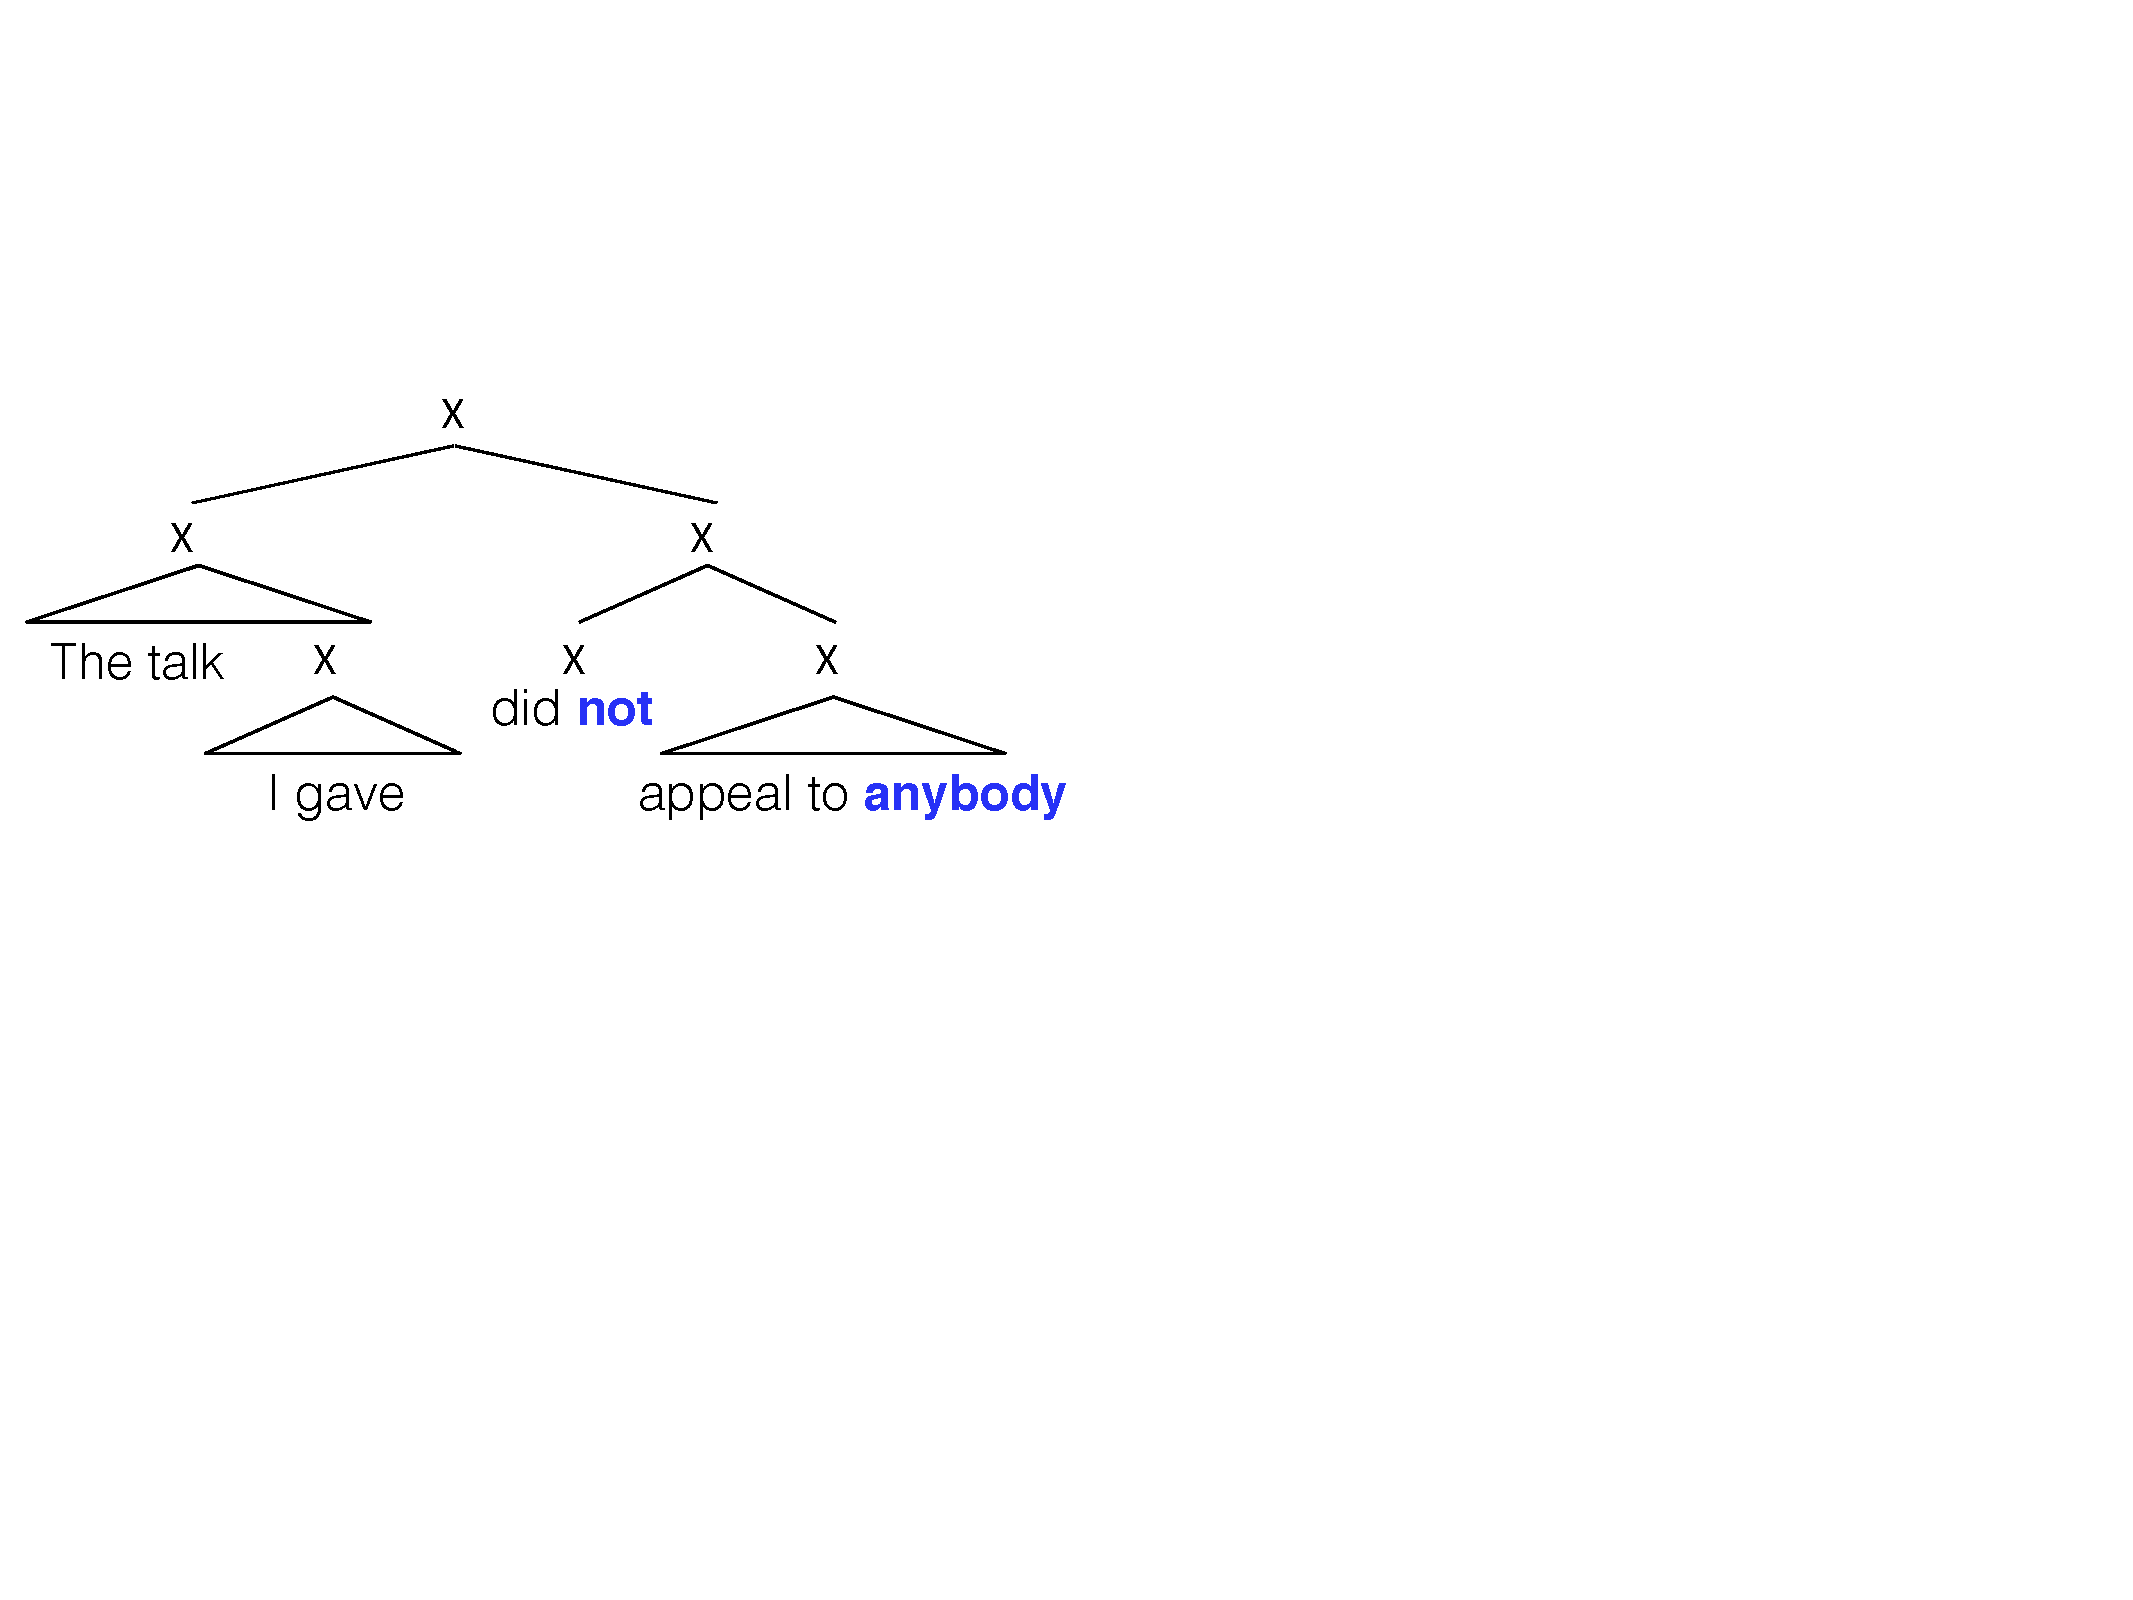
\includegraphics[width=0.9\textwidth]{trees/npi-licensed.pdf}
	\end{subfigure}
	\begin{subfigure}[b]{0.5\textwidth}
		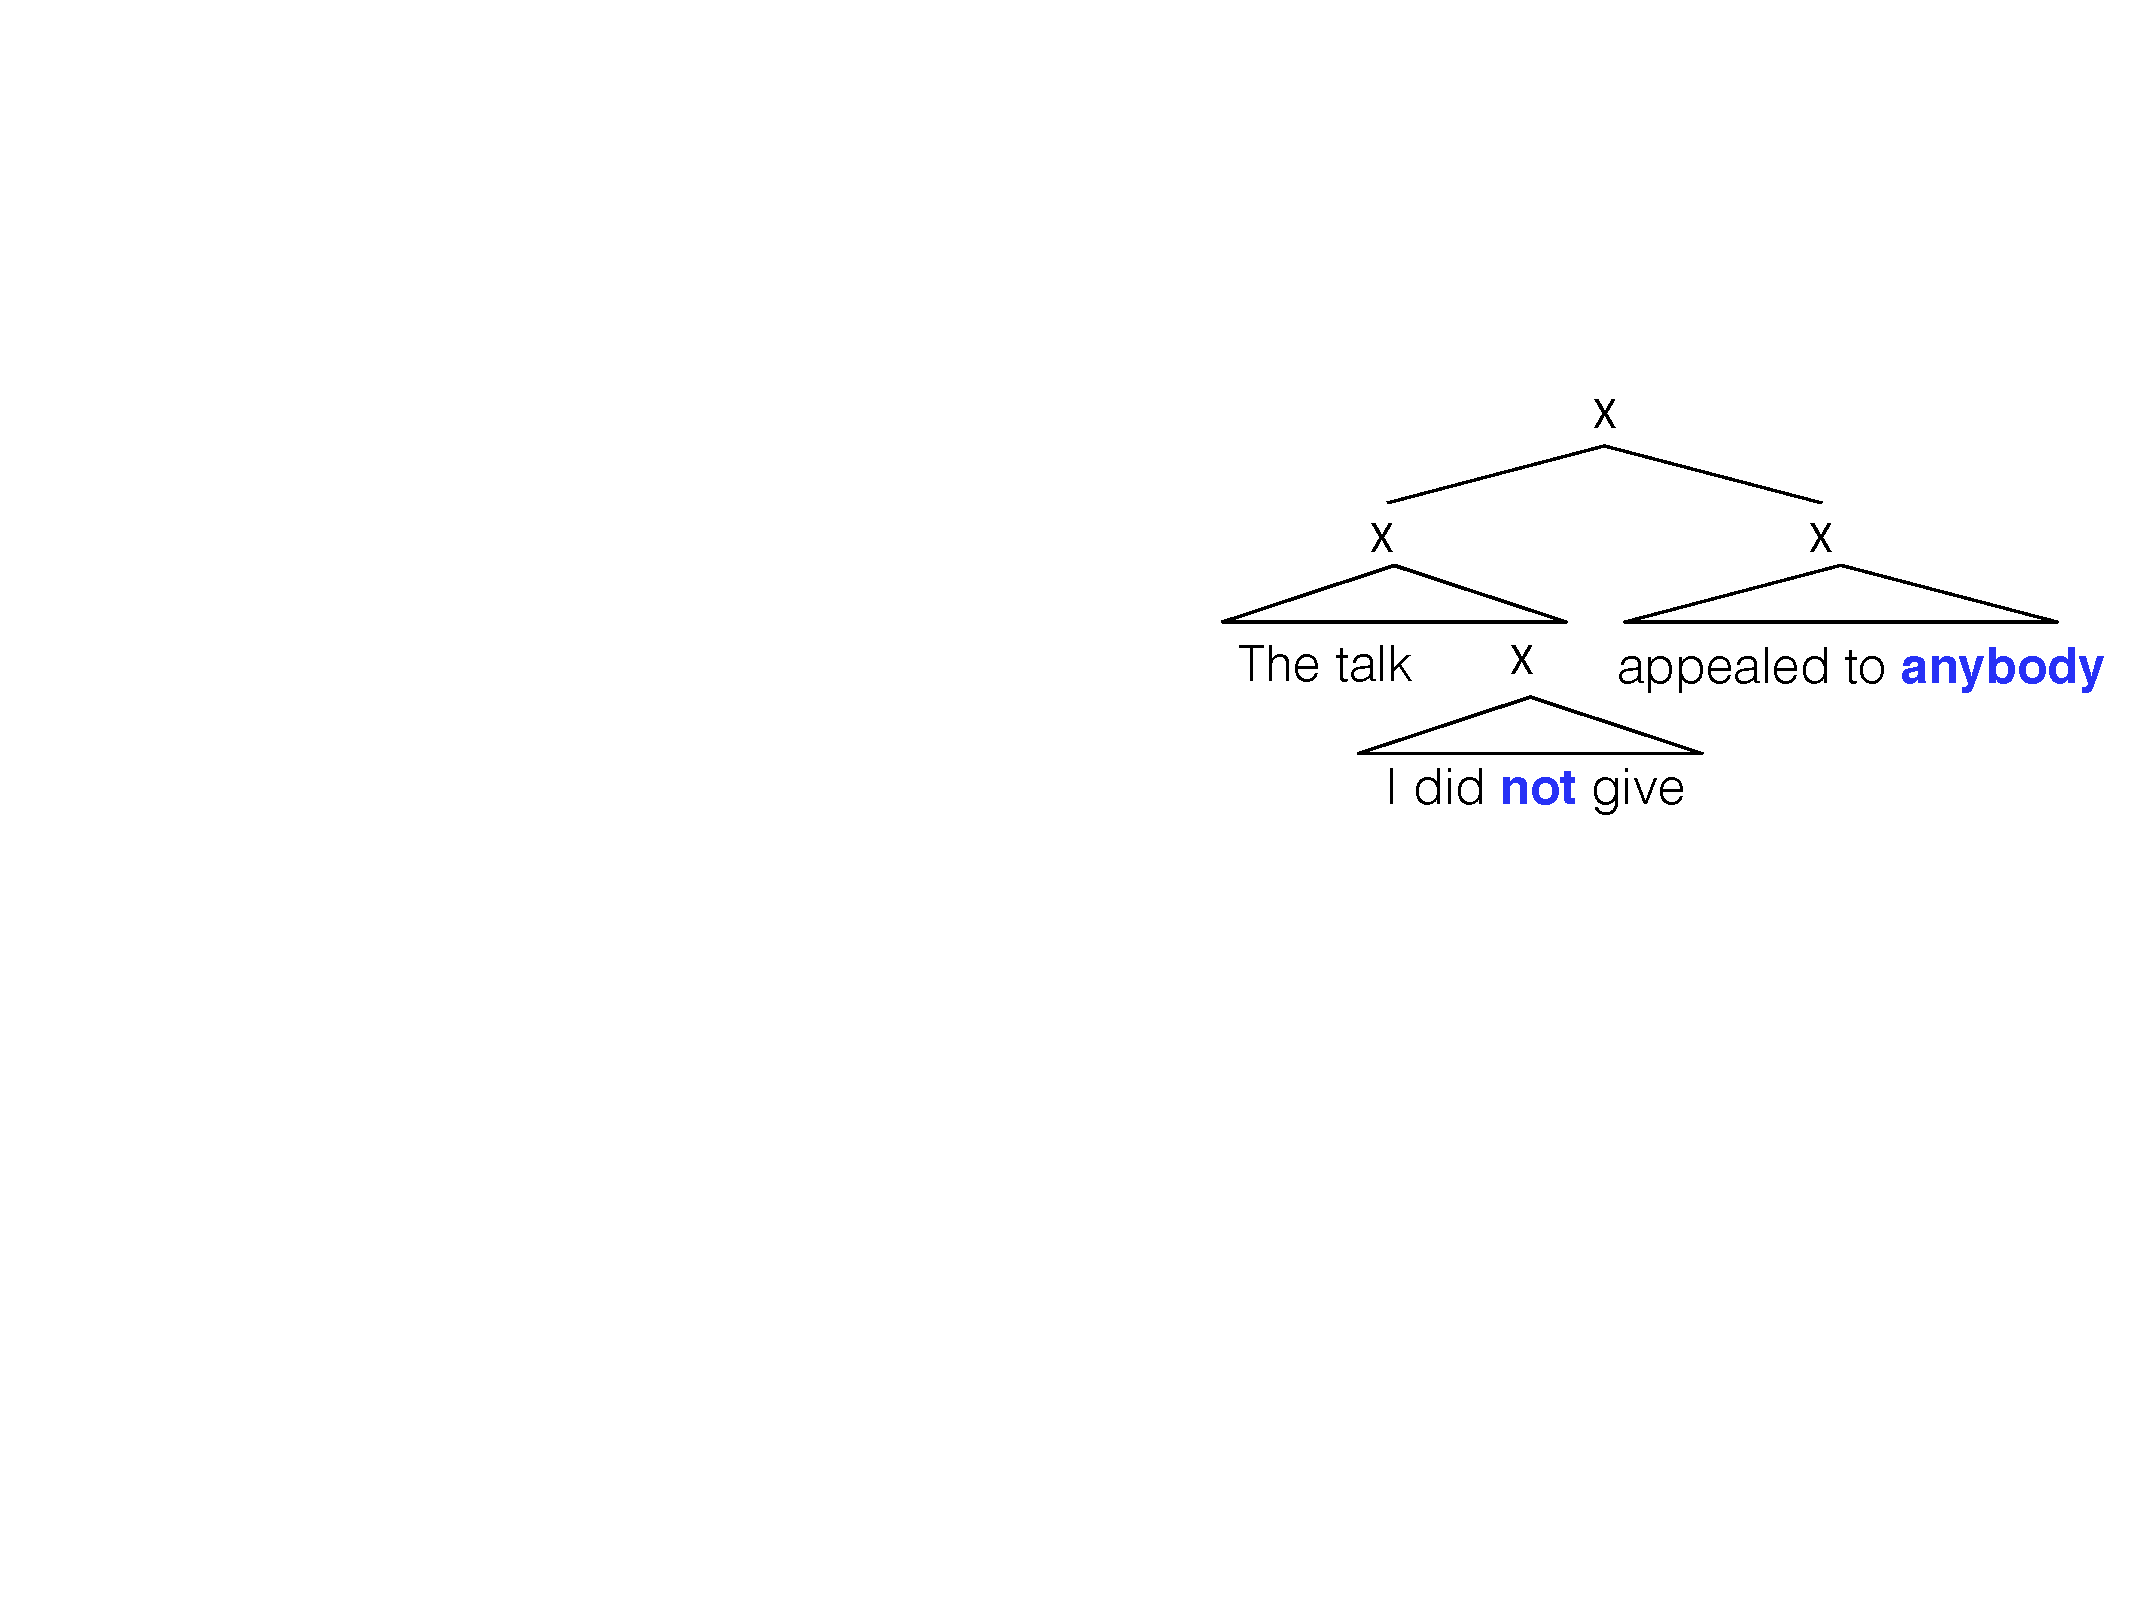
\includegraphics[width=0.9\textwidth]{trees/npi-unlicensed.pdf}
	\end{subfigure}
\caption{Hierarchical dependance of negative polarity items. Left shows the word \textit{anybody} in the licensing context of \textit{not}, while right shows the ungrammatical sentence where the word is not. Figure taken without permission from \cite{everaert2015structures}.}
\label{fig:trees-npi}
\end{figure}
Instead, it is argued, the constraints that govern this particular pattern depend on hierarchical structure: the word \textit{not} must `structurally precede' the word \textit{anybody} \citep{everaert2015structures}. Figure \label{ref:trees-npi} shows the constituent structure of both sentences. The explanation goes as follows (put this in my own words): \say{In sentence \ref{fig:trees-npi} (a) the hierarchical structure dominating \textit{not} also immediately dominates the hierarchical structure containing \textit{anybody}. In sentence \ref{fig:trees-npi} (b), by contrast, \textit{not} sequentially precedes \textit{anybody}, but the triangle dominating \textit{not} fails to also dominate the structure containing \textit{anybody}.}


\subsection{Controversy}
Theoretical syntax is rife with controversy, and wildly differing viewpoints exist. In fact, for each point made in our short discussion, the exact opposite point has been made as well:

\begin{itemize}
  \item Work in dependency grammar and other word-based grammar formalisms depart from the idea that lexical relations between individual words are more fundamental than constituents and their hierarchical organization \citep{tesniere1959elements,nivre2005dependency,hudson2010introduction}, and dispenses with the notion of constituents altogether.

  \item A recurring cause of controversy is the question whether hierarchical structure needs to be invoked in linguistic explanation. That is, whether the kind of analysis in figure \ref{fig:bird-tree}, with embedded constituents, is really fundamental to language. \citet{frank2012hierarchical} argue that a shallow analysis of sentences into immediate constituants with linear order but no hierachical structure\footnote{A structure reminiscent of that predicted in the task of \textit{chunking}, or shallow parsing.} is sufficient for syntactic theories, a claim that is vehemently rejected by \citet{everaert2015structures}.

  \item Research in cognitive neuroscience and psycholinguistics shows that human sentence processing is hierachical, giving evidence that processing crucially depends on the kind of structures introduced in the sections above \citep{hale2001earley,levy2008expectation,brennan2016abstract}. However, research also exists that shows that purely linear predictors are sufficient for modeling sentence comprehension, thus showing the exact opposite to be true \citep{conway2008neurocognitive,gillespie2011hierarchy,christiansen2012similar,gillespie2013against,frank2012hierarchical}.
\end{itemize}
Our work, however, takes a pragmatic position with respect to such questions: syntax, we assume, is whatever our dataset says it is. Whether language is hierachical or linear is a question that this thesis engages with from a statistical and computational standpoint.

\section{Parsing}
  Parsing is the task of predicting a tree $\y$ for a sentence $\x$. Probabilitic parsers solve this problem by learning a probabilistic model $p$ that describes a probability distribution over \textit{all} the possible parses $\y$ of sentences $\x$. This distribution quantifies the uncertainty over the syntactic analyses of the sentence, and can be used to make predictions by finding the trees with highest probability. A further benefit of the probabilistic formulation is that the uncertainty over the parses can be determined quantitatively by computing the entropy of the distribution, and qualitatively by obtaining samples from the distribution. This section describes the form that such probabilistic models take, and the data from which they are estimated.

  \subsection{Treebank}
    A treebank is a collection of sentences annotated with their grammatical structure that allows the estimation of statistical parsings models. The Penn Treebank \citep{marcus1993penn} is such a collection, consisting of sentences annotated with their constituency structure. Figure \ref{fig:tree-original} shows an example tree from this dataset and figure \ref{fig:tree-simplified} shows the tree after basic processing\footnote{This removes the functional tags and annotation of argument structure introduced in version 2 of the Penn Treebank \citep{marcus1994annotating}.}. Some of the models in this work require trees to be in \textit{normal form}: fully binary, but with unary branches at the terminals. Figure \ref{fig:tree-cnf} show the result of this (invertible) normalization, that is obtained by introduction of an empty dummy label $\varnothing$. Annotating the labels with left and right endpoints of the words they span results in the tree in figure \ref{fig:tree-cnf-spans}.

    A tree can be factorized into its parts: we can think of tree as a set of \textit{labeled spans}, or as a set of \textit{anchored rules}. A labeled span is a triple $(A, i, j)$ of a syntactic label $A$ from a labelset $\Lambda$ together the left and right endpoints $i$, $j$ that the label spans. An \textit{anchored rule} is a triple $(r, i, j)$ or four-tuple $(r, i, k, j)$, containing a rule $r$ in normal form with span endpoints $i$, $j$, and a split-point $k$ of the left and right child $r$ is not a lexical rule. For the difference, consider the two representations of the tree in figure \ref{fig:tree-cnf-spans} given in table \ref{tab:spans-rules}. These different factorizations will become relevant in chapter \ref{04-crf}.

    \begin{figure}

      \begin{subfigure}[b]{\textwidth}
        \center
        \begin{tikzpicture}[scale=.6]
          \Tree [.S
        [.SBAR-NOM-SBJ
          [.WHNP-1 What ]
          [.S [.NP-SBJ *T*-1 ] [.VP happened [.NP-TMP Friday ] ] ] ]
        [.VP
          was
          [.NP-PRD [.NP the worst ] [.PP of [.NP all worlds ] ] ] ]
        . ]

        \end{tikzpicture}
        \subcaption{Original Penn Treebank tree.}
    		\label{fig:tree-original}
      \end{subfigure}

      \begin{subfigure}[b]{\textwidth}
        \center
        \begin{tikzpicture}[scale=.6]
    		  \Tree [.S
        [.SBAR [.WHNP What ] [.S [.VP happened [.NP Friday ] ] ] ]
        [.VP
          was
          [.NP [.NP the worst ] [.PP of [.NP all worlds ] ] ] ]
        $.$ ]

        \end{tikzpicture}
        \tiny
        \subcaption{Function tags and traces removed.}
    		\label{fig:tree-simplified}
      \end{subfigure}

      \begin{subfigure}[b]{\textwidth}
        \center
        \begin{tikzpicture}[scale=.6]
    		  \Tree [.S
        [.SBAR [.WHNP What ] [.S+VP [.$\varnothing$ happened ] [.NP Friday ] ] ]
        [.$\varnothing$
          [.VP
            [.$\varnothing$ was ]
            [.NP
              [.NP [.$\varnothing$ the ] [.$\varnothing$ worst ] ]
              [.PP [.$\varnothing$ of ] [.NP [.$\varnothing$ all ] [.$\varnothing$ worlds ] ] ] ] ]
          [.$\varnothing$ . ] ] ]

        \end{tikzpicture}
        \tiny
        \subcaption{Converted to normal form.}
    		\label{fig:tree-cnf}
      \end{subfigure}

      \begin{subfigure}[b]{\textwidth}
        \center
        \begin{tikzpicture}[scale=.6]
    		  \Tree [.S:0-10
        [.SBAR:0-3
          [.WHNP:0-1 What ]
          [.S+VP:1-3 [.@:1-2 happened ] [.NP:2-3 Friday ] ] ]
        [.@:3-10
          [.VP:3-9
            [.@:3-4 was ]
            [.NP:4-9
              [.NP:4-6 [.@:4-5 the ] [.@:5-6 worst ] ]
              [.PP:6-9
                [.@:6-7 of ]
                [.NP:7-9 [.@:7-8 all ] [.@:8-9 worlds ] ] ] ] ]
          [.@:9-10 . ] ] ]

        \end{tikzpicture}
        \tiny
        \subcaption{In normal form with spans.}
    		\label{fig:tree-cnf-spans}
      \end{subfigure}

    \caption{Converting a treebank tree (withouth part-of-speech tags).}
    \label{fig:trees-ptb}
    \end{figure}

    \begin{table}[h]
      \center
      \small
      \bgroup  % increase vertical space
      \def\arraystretch{1.5}  % increase vertical space
      \begin{tabular}{l|l}
        Labeled spans & Anchored rules \\
        \hline
        (S, 0, 10)     & (S $\to$ SBAR $\varnothing$, 0, 3, 10)  \\
        (SBAR, 0, 3)   & (SBAR $\to$ WHNP S+VP, 0, 1, 3)  \\
        (WHNP, 0, 1)     & (WHNP $\to$ \textit{What}, 0, 1)  \\
        $\qquad\vdots$ & $\qquad\vdots$  \\
        ($\varnothing$, 9, 10)     & ($\varnothing$ $\to$ ., 9, 10)  \\
      \end{tabular}
      \caption{Two conceptions of the tree in \ref{fig:tree-cnf-spans}.}
      \label{tab:spans-rules}
      \egroup  % increase vertical space
    \end{table}


  \subsection{Models}
    The probabilistic model of a parser can be \textit{discriminative}, describing the conditional probability distribution $p(\y \mid \x)$, or \textit{generative}, describing the joint distribution $p(\x, \y)$. The form that the model takes is largely dictated by the algorithm used to build the parses.

    Transition-based methods formulate parsing as a sequence of shift-reduce decisions made by a push-down automaton that incrementally builds a tree. The design of the transition system determines whether the tree is constructed bottom-up, top-down, or otherwise\footnote{Post-order and pre-order tarversal, respectively.}, and determines whether the trees need to be in normal form. The probabilistic model is defined over the sequences of actions, and the probability distribution typically factorizes as the product of conditional distributions over the next action given the previous actions. This makes it a directed model that is \textit{locally normalized}.\footnote{With the exception of those approaches that instead define a Conditional Random Field over the action sequences \citep{andor2016globally}, in which case the model is defined over the globally normalized action sequences.}
    \begin{definition}{}
      A probalistic model $p(\x)$ over sequences $\x \in \mathcal{X}^n$ is \textit{locally normalized} if
      \begin{align*}
        p(\x)
          &= \prod_{i=1}^{n} p(x_i \mid x_{<i})  \\
          &= \prod_{i=1}^{n} \frac{ \Psi( x_{<i}, x_{i} ) }{ Z( x_{<i} ) },
      \end{align*}
      where $Z( x_{<i} ) = \sum_{x \in \mathcal{X}} \Psi( x_{<i}, x )$  is a local normalizer and $\Psi$ is a nonnegative scoring function: $\Psi( x_{<i}, x_{i} ) \geq 0$ for all $x_{<i}$ and $x$.
    \end{definition}
    Such a model is discriminative when the actions only build the tree, but can be made generative when word prediction is included in the action set.

    Chart based parsing, on the other hand, factorizes trees along their parts, and defines the probabilistic model over the shared substructures. Representing the model as the product of local parts greatly reduces the number of variables required to specify the full distribution, and allows the use of dynamic programming for efficient inference. Discriminitive models based on Conditional Random Fields (CRF) \citep{lafferty2001crf} follow this factorization: local functions independently predict scores for the parts, and the product of this score is normalized \textit{globally} by a normalizer that sums over the exponential number structures composable from the parts.
    \begin{definition}{}
      A probalistic model $p(\x)$ over sequences $\x \in \mathcal{X}^n$ is \textit{globally normalized} if
      \begin{align*}
        p(\x) = \frac{ \Psi( \x ) }{ Z },
      \end{align*}
      where $Z  = \sum_{\x \in \mathcal{X}^n} \Psi( \x )$ is a \textit{global} normalization term, and $\Psi (\x ) \geq 0$ for all $\x$. To allow efficient computation of the normalizer $Z$, the function $\Psi$ typically factors over parts of $x$ as $\Psi ( \x ) = \prod_{a=1}^A \psi (\x_a )$.
    \end{definition}
    Generative chart-based models, instead, estimate rule probabilities directly from a treebank. The probability of a tree is computed directly as the product of the probabilities of the rules that generate it, thus requiring no normalization.\footnote{In fact, this makes generative chart-based models directed, locally normalized models: they generate trees top-down by expanding localized normally rules.}.

    Either method have their advantages and disadvantages. The transition-based methods are fast, running in time linear in the sequence length, and allow arbitrary features that can condition on the entire sentence and the partially constructed derrivation. However, directed models with local normalization are known to suffer from the problem of label-bias \citep{lafferty2001crf}, and conditioning on large parts of the partial derivations prohibits exact inference, so that decoding can be done only approximately, either with greedy decoding or with beam search. The chart based methods, on the other hand, allow efficient exact inference, and the global training of the discriminative models [...something about learning from all substructures...]. The method is much slower, however, running in time cubic in the sentence length for normal form trees \footnote{And slower for trees that are not in normal form.} and linear in the size of the grammar\footnote{Giving a total time complexity of $O(n^3|G|)$.}, and the strong factorization of the structure, which makes the exact inference tractable, also means that features can condition only on small parts instead of large substructures.

    A general challenge for greedy transition is that their training is highly local: they are only exposed to the individual paths that generate the example tree, which is a mere fraction of all the possible paths that the model is defined over.\footnote{One way to answer to this challenge is to use use a dynamic oracle during training \citep{goldberg2013dynamic}, also called exploration \citep{ballesteros2016exploration,stern2017minimal}, which allow the model to explore paths that deviate from the single gold path in a principled way. The approach can be considered an instance of imitation learning \citep{vlachos2012imitation,he2012imitation}. In constituency parsing, dynamic oracles can produce substantial improvements performance \citep{ballesteros2016exploration}, but they must be custom designed for each transition system \citep{klein2018reinforce}. However, we do not consider this directions in this thesis.} Compare this with a globally normalized model, where the factorization over parts lets the model learn from an example tree about all the trees that share substructure.

    In this thesis we investigate models where the scoring function $\Psi$, or its factorized version $\psi$, is implemented with neural networks. Chapter \ref{03-rnng} describes a locally normalized transition-based model that has a discriminative and generative formulation, and chapter \ref{04-crf} introduces a globally normalized, discriminative chart-based parser.


  \subsection{Metrics}
    The standard evaluation for parsing is the Parseval metric \citep{black1991parseval}, which measures the number of correctly predicted labeled spans. Let $\mathcal{R}$ be the set of labeled spans of the gold reference trees, and let $\mathcal{P}$. The metric is defined as the harmonic mean, or $F_1$ measure, of the labelling recall $R$ and precison $P$:
    \begin{align}
      \label{eq:fscore}
      F_1 = \frac{2 PR}{P + R}.
    \end{align}
    The recall is the fraction of reference spans that are predicted correctly
    \begin{align*}
      R = \frac{|\mathcal{R} \cap \mathcal{S}|}{|\mathcal{R}|},
    \end{align*}
    and the precision is the fraction of the source spans that is correct
    \begin{align*}
      P = \frac{|\mathcal{R} \cap \mathcal{S}|}{|\mathcal{S}|}.
    \end{align*}
    The cannonical implementation of the Parseval metric is \verb!EVALB! \citep{sekine1997evalb}.


\section{Language models}
  A language model is a probability distribution over sequences of words. There are many ways to design such a model, and many datasets to estimate them from. This section focusses on those that are relevant to the models in this thesis.

  \subsection{Models}
    A language model is a probabilistic model $p$ that assigns probabilities to sentences, or more formally, to sequences $\x \in \mathcal{X}^{*}$ of any length over a finite vocabulary. Factorizing the probability of a single sequence $\x \in \mathcal{X}^m$ over its timesteps gives the directed model:
    \begin{align}
      \label{eq:lm-factorized}
      p( \x )
        &= \prod_{i=1}^m p(x_i \mid x_{<i}).
    \end{align}
    This distribution can be approximated by lower order conditionals that condition on smaller, fixed-size, history, by making the Markov assumption assumption that
    \begin{align*}
      p(x_i \mid x_{<i}) = p(x_i \mid x_{i-j-1}^{i-1}).
    \end{align*}
    This is the approach taken by $n$-gram language models. The lower order conditionals can be estimated directly by smoothing occurence counts \citep{chen1999empirical,kneser1995improved}, or they can be estimated by locally normalized scores $\Psi(x_{i-j-1}^{i-1}, x_i)$, given by a parametrized function $\Psi$. This function can be log-linear or a non-linear neural network \citep{rosenfeld1996loglinear,bengio2003neural}. The lower order approximation can also be dispensed with, making the model more epressive, but the estimation problem much harder. Language models based on recurrent neural networks (RNNs) follow this approach by using functions that compute scores $\Psi(x_{<i}, x_i)$ based on the entire history \citep{mikolov2010recurrent}. These models, and in particular the approaches based on the LSTM variant of the RNN, have shown to be remarkably effective and substantially improve over the above methods to give the current state of the art \citep{zaremba2014recurrent,jozefowicz2016exploring}.\footnote{Although recent work shows that the effective memory depth of RNN models is much smaller than the unbounded history suggests: \citet{chelba2017n} show that, in the perplexity they assign to test data, an RNN with unbounded history can be approximated very well by an RNN with bounded history. To be precise: a neural $n$-gram language model, with the fixed-size history encoded by a bidirectional RNN, is equivalent to an RNN with unbounded history for $n=13$, and to an RNN that is reset at the start of sentences for $n=9$. This finding is consistent accross dataset sizes.} Other neural network architectures based on convolutions \citep{kalchbrenner2014convolutional} and stacked feedforward networks with `self-attention' \citep{vaswani2017attention} have been succesfully applied to language modelling with unbounded histories as well.

    Alternatively, a language model can be obtained by marginalizing a structured latent variable $h$ in a joint model $p(\x, h)$:
    \begin{align}
      \label{eq:lm-latent}
      p( \x ) = \sum_{h \in \mathcal{H}} p(\x, h).
    \end{align}
    The structure of $h$ allows this joint distribution to be factorized in a ways very much unlike that of equation \ref{eq:lm-factorized}. Such language models are defined for example by a Probabilistic Context Free Grammar (PCFG), in which case $h$ is a tree, and a Hidden Markov Model (HMM), in which case $h$ is a sequence of tags. The strong independence assumptions of these models allows the marginalization to be computed efficiently, but also disallows the models to capture dependencies in $\x$, which is precisely what we want from a language model. The recurrent neural network grammar (RNNG) model introduced in chapter \ref{03-rnng} also defines a language model through a joint distribution, but that model is factorized as a sequential generation process over both the latent structure $h$ and the observed sequence $\x$, which makes it a competitive language model, but at the price of losing efficient exact marginalization.

    Some other language models that incorporate syntax: language models obtained from top-down parsing with a PCFG \citep{roark2001probabilistic}; syntactic extensions of $n$-gram models with count-based and neural network estimation \citep{chelba2000structured,emami2005neural}; and an method that is reminiscent of $n$-gram methods, but based on arbitrary overlapping tree fragments \citep{pauls2012treelets}.

  \subsection{Data}
    Language models enjoy the benefit that they require no labeled data; any collection of tokenized text can be used for training. In this work we focus on English language datasets. The tokens from Penn Treebank have long been a popular dataset for this task. More recently has seen the introduction of datasets of much greater size, such as the One Billion Word Benchmark \citep{chelba2013one} that consists of news articles, and datasets that focus on long-distance dependencies, such as the Wikitext datasets \citep{merity2016pointer} that consists of Wikipedia articles grouped into paragraphs.

  \subsection{Metrics}
    The standard metric to evaluate a language model is the \textit{perplexity} that it assigns to held out data. The lower the perplexity, the better the model. Perplexity is an information theoretic metric that corresponds to an exponentiated estimate of the model's entropy, measured in nats, and was introduced for this purpose by \citet{jelinek1997information}\footnote{According to \citep{chelba2017n}.}. The metric can be interpreted as the average number of guesses needed by the model to predict each word from its left context.

    \begin{definition}{} The perplexity of a language model $p$ on a sentence $\x$ of length $m$ is defined as
    \begin{align*}
      \exp \Bigg\{ - \frac{1}{m} \log p( \x ) \Bigg\}.
    \end{align*}
    The perplexity on a set of sentences $\{ \x^{(1)}, \dots, \x^{(N)} \}$ is defined as the exponentiated mean over all words together:
    \begin{align*}
      \exp \Bigg\{ - \frac{1}{M} \sum_{i=1}^N \log p( \x^{(i)} ) \Bigg\},
    \end{align*}
    where $M = \sum_{i=1}^N m_i$ is the sum of all the sentence lengths $m_i$.
    \end{definition}

   The appeal of perplexity is that it is an aggregate metric, conflating different causes of succes when predicting the next word. This conflation is also its main shortcoming, making it hard to determine whether the model has robustely learned high-level linguistic patterns such as those described in syntactic and semantic theories. For this reason, alternative methods have been proposed to evaluate language models: evaluation with adversarial examples \citep{smith2012adversarial}; prediction of long distance subject-verb agreement \citep{linzen2016syntax}; and eliciting syntactic acceptability judgments \citep{linzen2018targeted}. Chapter \ref{06-syneval} discusses these alternatives in greater detail, and demonstrates evalution with the method proposed in \citep{linzen2018targeted}.


\section{Neural networks}

  In this thesis we use neural networks to parametrize probability distributions. We consider a neural network as an abstraction that denotes a certain type of parametrized differentiable function, and use various kinds. Let $x$ be a word from a finite vocabulary $\mathcal{X}$, and let $\vecx$ and $\vecy$ be vectors in respectively $\reals^{n}$ and $\reals^{m}$.

  \begin{definition}{} A \textit{word embedding} is vector representation of a word, assigned by an embeding function $\embed$ that takes elements from $\mathcal{X}$ to $\reals^{n}$:
  \begin{align*}
    \vecx = \embed( x ).
  \end{align*}
  The function can be a simple lookup table, or a more elaborate function that depends for example on the orthography of the word.
  \end{definition}

  \begin{definition}{} A \textit{feedforward neural network} is a parametrized function $\ff$ from $\reals^{n}$ to $\reals^{m}$:
  \begin{align*}
    \vecy = \ff( \vecx ).
  \end{align*}
  Internally, the function computes an affine transformation followed by an elementwise application of a nonlinear function, repeatedly. The number of repetitions is refered to as the number of layers of the network.
  \end{definition}

  \begin{definition}{} A \textit{recurrent neural network} (RNN) is a parametrized function $\rnn$ that takes a sequence of vectors $\mathbf{X} = [ \vecx_1, \vecx_2, \dots, \vecx_k ]$, each in $\reals^{n}$,\footnote{Compactly represented as a matrix $\mathbf{X} \in \reals^{n \times k}$.} and produces a sequence of output vectors $[\vecy_1, \vecy_2, \dots,\vecy_n]$ each in $\reals^{m}$:
  \begin{align*}
    [\vecy_1, \vecy_2, \dots, \vecy_k] = \rnn( \mathbf{X} ).
  \end{align*}
  Each vector $\vecy_i$ is a function of the vectors $[\vecx_1, \vecx_2, \dots, \vecx_i ]$, for which reason we refer to the vector $\vecy_i$ as a context-dependent \textit{encoding} of the vector $\vecx_i$. An $\rnn$ can be applied to the input sequence in reverse. This makes each $\vecy_i$ a function of the vectors $[\vecx_i, \vecx_{i+1}, \dots, \vecx_k ]$. We denote the output of the forward direction with $\fw$ and the output of the backward direction with $\bw$.
  \end{definition}

  \begin{definition}{} An RNN is \textit{bidirectional} when it combines the output of an RNN that runs in the forward direction, with the output of an RNN that  runs in the backward direction. Combining their output vectors by concatenation gives for each position a vector $\h_i = [ \fw_i; \bw_i ]$ that is a function of the entire input sequence.
  \end{definition}

  \begin{definition}{} An LSTM \citep{hochreiter1997long} is a particular way to implement the internals of the RNN function. It is the only type of RNN used in this work, and we use the two names exchangeably.
  \end{definition}

  % \begin{itemize}
  %
  %   \item A \textit{word embedding} is vector representation of a word, assigned by an embeding function $\embed$ that takes elements from $\mathcal{X}$ to $\reals^{n}$:
  %   \begin{align*}
  %     \vecx = \embed( x ).
  %   \end{align*}
  %   The function can be a simple lookup table, or a more elaborate function that depends for example on the orthography of the word.
  %
  %   \item A \textit{feedforward neural network} is a parametrized function $\ff$ from $\reals^{n}$ to $\reals^{m}$:
  %   \begin{align*}
  %     \vecy = \ff( \vecx ).
  %   \end{align*}
  %   Internally, the function computes an affine transformation of the input vector followed by an elementwise application of a nonlinear function, repeatedly. The number of repetitions is refered to as the number of layers of the network.
  %
  %   \item A \textit{recurrent neural network} (RNN) is a parametrized function $\rnn$ that takes a sequence of vectors $\vecx = [ \vecx_1, \vecx_2, \dots, \vecx_n ]$ from $\reals^{n}$ and produces a sequence of output vectors $[\vecy_1, \vecy_2, \dots,\vecy_n]$ in $\reals^{m}$:
  %   \begin{align*}
  %     [\vecy_1, \vecy_2, \dots, \vecy_n] = \rnn( \vecx ).
  %   \end{align*}
  %   Each vector $\vecy_i$ is a function of the vectors $[\vecx_1, \vecx_2, \dots, \vecx_i ]$, for which reason we refer to the vector $\vecy_i$ as a context-dependent \textit{encoding} of the vector $\vecx_i$. An $\rnn$ can be applied to the input sequence in reverse. This makes each $\vecy_i$ a function of the vectors $[\vecx_i, \vecx_{i-1}, \dots, \vecx_1 ]$. We denote the output of the forward direction with $\fw$ and the output of the backward direction with $\bw$.
  %
  %   \item An RNN is \textit{bidirectional} when it combines the output of an RNN that runs in the forward direction, with the output of an RNN that runs in the backward direction. Combining their output vectors by concatenation gives for each position a vector $\h_i = [ \fw_i; \bw_i ]$ that is a function of the entire input sequence.
  %
  %   \item An LSTM \citep{hochreiter1997long} is a particular way to implement the RNN function. It is the only type of RNN used in this work, and we use the two names exchangeably.
  %
  % \end{itemize}
